%%%%%%%%%%%%%%%%%%%%%%%%%%%%%%%%%%%%%%%%%
% Wenneker Assignment
% LaTeX Template
% Version 2.0 (12/1/2019)
%
% This template originates from:
% http://www.LaTeXTemplates.com
%
% Authors:
% Vel (vel@LaTeXTemplates.com)
% Frits Wenneker
%
% License:
% CC BY-NC-SA 3.0 (http://creativecommons.org/licenses/by-nc-sa/3.0/)
% 
%%%%%%%%%%%%%%%%%%%%%%%%%%%%%%%%%%%%%%%%%

%----------------------------------------------------------------------------------------
%	PACKAGES AND OTHER DOCUMENT CONFIGURATIONS
%----------------------------------------------------------------------------------------

\documentclass[11pt]{scrartcl} % Font size
\newcommand{\comment}[1]{}
%%%%%%%%%%%%%%%%%%%%%%%%%%%%%%%%%%%%%%%%%
% Wenneker Assignment
% Structure Specification File
% Version 2.0 (12/1/2019)
%
% This template originates from:
% http://www.LaTeXTemplates.com
%
% Authors:
% Vel (vel@LaTeXTemplates.com)
% Frits Wenneker
%
% License:
% CC BY-NC-SA 3.0 (http://creativecommons.org/licenses/by-nc-sa/3.0/)
% 
%%%%%%%%%%%%%%%%%%%%%%%%%%%%%%%%%%%%%%%%%

%----------------------------------------------------------------------------------------
%	PACKAGES AND OTHER DOCUMENT CONFIGURATIONS
%----------------------------------------------------------------------------------------

\usepackage{amsmath, amsfonts, amsthm} % Math packages

\usepackage{listings} % Code listings, with syntax highlighting

\usepackage[english]{babel} % English language hyphenation

\usepackage{graphicx} % Required for inserting images
\graphicspath{{Figures/}{./}} % Specifies where to look for included images (trailing slash required)

\usepackage{booktabs} % Required for better horizontal rules in tables

\numberwithin{equation}{section} % Number equations within sections (i.e. 1.1, 1.2, 2.1, 2.2 instead of 1, 2, 3, 4)
\numberwithin{figure}{section} % Number figures within sections (i.e. 1.1, 1.2, 2.1, 2.2 instead of 1, 2, 3, 4)
\numberwithin{table}{section} % Number tables within sections (i.e. 1.1, 1.2, 2.1, 2.2 instead of 1, 2, 3, 4)

\setlength\parindent{0pt} % Removes all indentation from paragraphs

\usepackage{enumitem} % Required for list customisation
\setlist{noitemsep} % No spacing between list items

%----------------------------------------------------------------------------------------
%	DOCUMENT MARGINS
%----------------------------------------------------------------------------------------

\usepackage{geometry} % Required for adjusting page dimensions and margins

\geometry{
	paper=a4paper, % Paper size, change to letterpaper for US letter size
	top=2.5cm, % Top margin
	bottom=3cm, % Bottom margin
	left=3cm, % Left margin
	right=3cm, % Right margin
	headheight=0.75cm, % Header height
	footskip=1.5cm, % Space from the bottom margin to the baseline of the footer
	headsep=0.75cm, % Space from the top margin to the baseline of the header
	%showframe, % Uncomment to show how the type block is set on the page
}

%----------------------------------------------------------------------------------------
%	FONTS
%----------------------------------------------------------------------------------------

\usepackage[utf8]{inputenc} % Required for inputting international characters
\usepackage[T1]{fontenc} % Use 8-bit encoding

\usepackage{fourier} % Use the Adobe Utopia font for the document

%----------------------------------------------------------------------------------------
%	SECTION TITLES
%----------------------------------------------------------------------------------------

\usepackage{sectsty} % Allows customising section commands

\sectionfont{\vspace{6pt}\centering\normalfont\scshape} % \section{} styling
\subsectionfont{\normalfont\bfseries} % \subsection{} styling
\subsubsectionfont{\normalfont\itshape} % \subsubsection{} styling
\paragraphfont{\normalfont\scshape} % \paragraph{} styling

%----------------------------------------------------------------------------------------
%	HEADERS AND FOOTERS
%----------------------------------------------------------------------------------------

\usepackage{scrlayer-scrpage} % Required for customising headers and footers

\ohead*{} % Right header
\ihead*{} % Left header
\chead*{} % Centre header

\ofoot*{} % Right footer
\ifoot*{} % Left footer
\cfoot*{\pagemark} % Centre footer
 % Include the file specifying the document structure and custom commands

%----------------------------------------------------------------------------------------
%	TITLE SECTION
%----------------------------------------------------------------------------------------

\title{	
	\normalfont\normalsize
	\textsc{Rutgers University, New Brunswick}\\ % Your university, school and/or department name(s)
	\vspace{25pt} % Whitespace
	\rule{\linewidth}{0.5pt}\\ % Thin top horizontal rule
	\vspace{20pt} % Whitespace
	{\huge Mazes}\\ % The assignment title
	\vspace{12pt} % Whitespace
	\rule{\linewidth}{2pt}\\ % Thick bottom horizontal rule
	\vspace{12pt} % Whitespace
}

\author{\LARGE Eshaan Gandhi, Siddarth Mandayam} % Your name

\date{\normalsize\today} % Today's date (\today) or a custom date

\begin{document}

\maketitle % Print the title

%----------------------------------------------------------------------------------------
%	FIGURE EXAMPLE
%----------------------------------------------------------------------------------------
\comment{
\section{Image Interpretation}

\begin{figure}[h] % [h] forces the figure to be output where it is defined in the code (it suppresses floating)
	\centering
	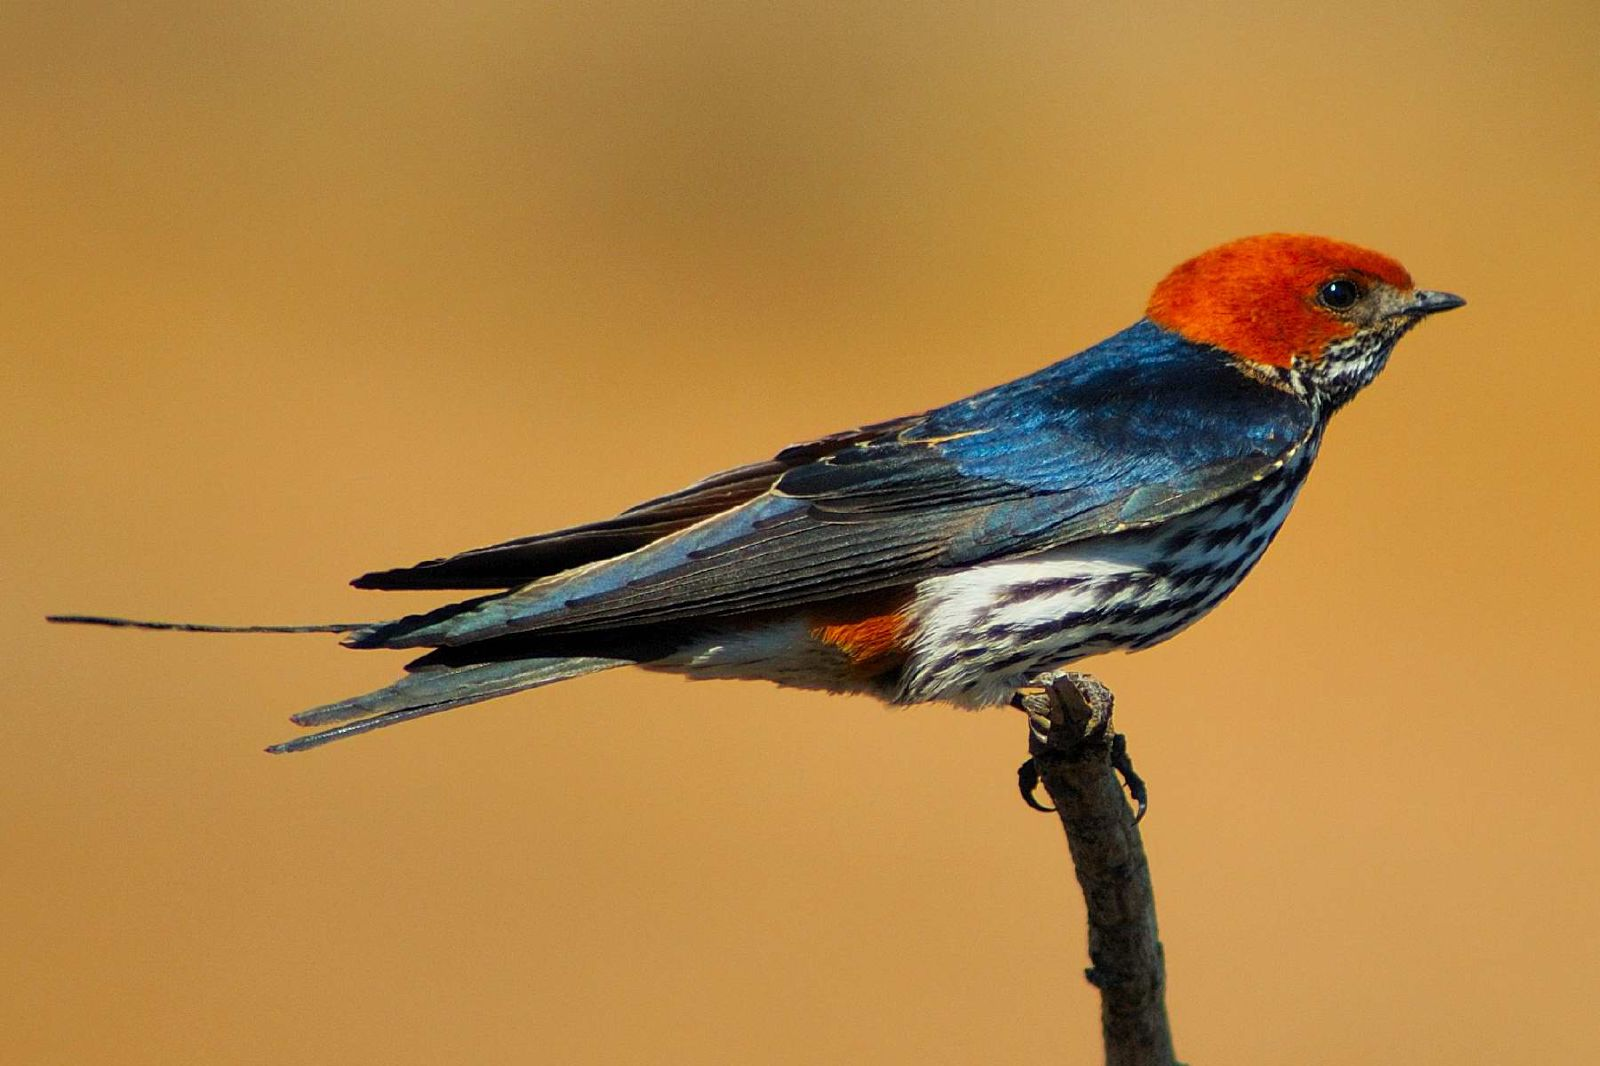
\includegraphics[width=0.5\columnwidth]{swallow.jpg} % Example image
	\caption{European swallow.}
\end{figure}

%------------------------------------------------
}%commented out

\section{The maze is on fire}

\subsection{Testing out our environment}
What I mean by testing out our environment is that we wanted to demonstrate the maze being generated with a given block density $\rho$. We also wanted to demonstrate the placement of fire and initial path to the target.\\

So we first generated a few maps with varying levels of block-density as demonstrated by the graphics below. \\

%Add image of the empty mazes

Next we would like to confirm that one element at random gets set on fire as demonstrated by the graphics below. \\

%add image of fire and fire spreadying for flammability q

\subsection{Strategy 1}
So strategy 1 is a naive way to go about this, but would not require that many resource to go about it. It simply does not care about the fire, and the person does get burned pretty often. Here is the strategy statement in detail. At the start of the maze, wherever the fire is, we solve for the shortest path from upper left to lower right, and follow  it  until the  agent  exits  the  maze  or  burns.   This  strategy  does  not  modify  its  initial  path  as  the  fire changes.
\vspace{2em}\\
We were tasked in generating a plot of ‘average successes vs flammability $q$’. To do that we had to run our program for strategy 1 $n$ number of times. In the assignment document, the minimum number is 10, but we realized that these many tries does not represent the true statistic well because of variance. So we in turn ran the maze a 1000 times for 11 values of q - 0 .. 1. \\
\pagebreak\\
We have recorded our finding in the table above.\\
\begin{table}[]
\caption{Strategy 1}
\begin{tabular}{|l|l|l|l|}
\hline
\textbf{Valid iterations} & \textbf{q} & \textbf{s - number of succeesses} & \textbf{u - number of times the agent got burned} \\ \hline
1000 & 0.0   & 736 & 264 \\ \hline
1000 & 0.1 & 556 & 444 \\ \hline
1000 & 0.2 & 375 & 625 \\ \hline
1000 & 0.3 & 316 & 684 \\ \hline
1000 & 0.4 & 181 & 819 \\ \hline
1000 & 0.5 & 162 & 838 \\ \hline
1000 & 0.6 & 95  & 905 \\ \hline
1000 & 0.7 & 75  & 925 \\ \hline
1000 & 0.8 & 59  & 941 \\ \hline
1000 & 0.9 & 42  & 958 \\ \hline
1000 & 1.0   & 37  & 963 \\ \hline
\end{tabular}
\end{table}\\
We then plot our findings in a line graph below. 
%insert line graph below
\comment{
\begin{figure}
 	\centering
  	\includegraphics*[scale=0.8]{strategy1.png}
	%\caption{Recursion tree and analysis}
	\label{fig:example}
 \end{figure}
\\This is our analysis for the 1st strategy. \\
}

\subsection{Strategy 2}
So strategy 2 is a better way to go about this than strategy 1, but would require more resource than strategy 1. It recomputes it's path every time it makes a step. Here is the strategy statement in detail. At every time step, we re-compute the shortest path from the agent’s current position to the goal position, based on  the  current  state  of  the  maze  and  the  fire.  We then follow  this  new  path  one  time  step,  then  re-compute.   This strategy constantly re-adjusts its plan based on the evolution of the fire.  If the agent gets trapped with no path to the goal, it dies.
\vspace{2em}\\
We were tasked in generating a plot of ‘average successes vs flammability $q$’. To do that we had to run our program for strategy 2 $n$ number of times. In the assignment document, the minimum number is 10, but we realized that these many tries does not represent the true statistic well because of variance. So we in turn ran the maze a 1000 times for 11 values of q - 0 .. 1. \\
\pagebreak\\
We have recorded our finding in the table above.\\
\begin{table}[]
\begin{tabular}{|l|l|l|l|}
\hline
\textbf{Valid iterations} & \textbf{q} & \textbf{s - number of succeesses} & \textbf{u - number of times the agent got burned} \\ \hline
1000 & 0.0   & 913 & 87  \\ \hline
1000 & 0.1 & 706 & 294 \\ \hline
1000 & 0.2 & 451 & 549 \\ \hline
1000 & 0.3 & 353 & 647 \\ \hline
1000 & 0.4 & 241 & 759 \\ \hline
1000 & 0.5 & 172 & 828 \\ \hline
1000 & 0.6 & 134 & 886 \\ \hline
1000 & 0.7 & 70  & 930 \\ \hline
1000 & 0.8 & 68  & 932 \\ \hline
1000 & 0.9 & 46  & 954 \\ \hline
1000 & 1.0 & 52  & 948 \\ \hline
\end{tabular}
\end{table}\\
We then plot our findings in a line graph below. 
%insert line graph below
\comment{
\begin{figure}
 	\centering
  	\includegraphics*[scale=0.8]{strategy2.png}
	%\caption{Recursion tree and analysis}
	\label{fig:example}
 \end{figure}
\\This is our analysis for the 2nd strategy.
}
\\

\subsection{Strategy 3 - GTFO! (Graph The Fire Out)}
We then wanted to try out our own strategy. The problem with strategy 1 and strategy 2 is that it does not take into consideration changing state of the maze and future state of the maze respectively. So we thought we could simulate part of the maze and see how we do. We started out simulating the whole maze but that would just mean that the fire engulfs the whole maze and finding a path is near impossible. So we simulate a part of the maze and try to find a path. We then take that path in the original maze and would likely make it. If we do make it, then we simulate it again. This strategy takes the future states into account, moves a bit, and then takes into account the changing state of the fire. \vspace{2em}\\

Well we found out it does very well for when the fire is not spreading rapidly, but does rather poorly when the fire is pretty fast. Here is the data.\\
\vspace{2em}\\
\begin{table}[]
\begin{tabular}{|l|l|l|l|}
\hline
\textbf{Valid iterations} & \textbf{q - flammability rate} & \textbf{s - succeesses} & \textbf{u - Times the agent got burned} \\ \hline
1000 & 0.0   & 919 & 81  \\ \hline
1000 & 0.1 & 651 & 349 \\ \hline
1000 & 0.2 & 453 & 547 \\ \hline
1000 & 0.3 & 337 & 663 \\ \hline
1000 & 0.4 & 214 & 786 \\ \hline
1000 & 0.5 & 159 & 841 \\ \hline
1000 & 0.6 & 99  & 901 \\ \hline
1000 & 0.7 & 74  & 926 \\ \hline
1000 & 0.8 & 54  & 946 \\ \hline
1000 & 0.9 & 58  & 942 \\ \hline
1000 & 1.0   & 39  & 961 \\ \hline
\end{tabular}
\end{table}

%Note - We use a numpy 2-d array to represent our maze and this should be well documented in our code. \\
\subsection{Comparison}
If we look at all the data, we can conclude that strategy 2 might be the best strategy, but it is very computationally expensive. We calculate the BFS path at every step. Our player might not have that kind of time when the fire is spreading fast.\vspace{2em}\\
For the first strategy the time complexity is $O(b^{d+1})$ as we only compute BFS once. Where $b = 4$ as we are computing 4 adjacent nodes.\vspace{2em}\\
Now if we look at Strategy 2, we are doing BFS on every movement. That is $O(k(b^{d+1})$ In real time we probably don't have that much time to make a decision in a maze that may be burning pretty fast.\vspace{2em}\\
The third strategy is simulating the future fire. If we were in a maze, we could kind of eyeball what the fire would look like. Simulating fire is not that computationally heavy and we only have to do BFS a fraction of the time we do it in strategy 2. We also get very similar results if we go about strategy 3. 

\subsection{Note on dimensions}
As we mentioned the time complexities of all three methods, this becomes very computationally expensive for the computer. I also wanted to generate a lot more maps than 10 as that removes variance. There are a number of times when we generate a map and it is rejected as there is not even an initial way to the goal. For these reasons, I chose a non-trivial dimension that is fast enough to run more than 1000 times for each value of $q$ and also large enough for the variance to not produce too much change how many successes we get. 

\end{document}
